\documentclass{article}
\usepackage[utf8]{inputenc}
\usepackage[T1]{fontenc}
\usepackage{hyphenat}
\usepackage{amsmath}
\usepackage{natbib}
%\bibliographystyle{dinat}
\bibliographystyle{abbrv}
\usepackage{multirow}
\usepackage{multicol}
\usepackage{booktabs}
\usepackage{graphicx}
\usepackage[labelformat=simple]{subcaption}
\renewcommand\thesubfigure{(\alph{subfigure})}
\usepackage{mwe}
\usepackage{afterpage}
\usepackage[export]{adjustbox}
\hyphenation{Mathe-matik wieder-gewinnen}

\title{\Huge A simple AutoML system \\
        \vspace{0.3cm} \large Building an Automated Machine Learning system to predict delay of airplanes}
\author{Patrick Kaiser, Jonas Schweisthal}
\date{29.03.2021}


\begin{document}

\begin{titlepage}
   \begin{center}
       \textsc{\Huge{ A simple AutoML system} \\
                \vspace{0.3cm} \large  Building an Automated Machine Learning system to predict delay of airplanes}
   \end{center}
   \begin{figure}[h]
       \centering
       
\includegraphics[width = 7cm]{image/SiegelLMU.jpg}
   \end{figure}
   \begin{center}
       \text{Assignment AutoML}\\ 
       \text{LMU München} \\
       \vspace{0.7cm}
       \text{Patrick Kaiser, Jonas Schweisthal}\\
       \vspace{0.3cm}
       \text{29.03.2021}
   \end{center}
\end{titlepage}

\begin{abstract}
In this article an AutoML system is introduced for predicting the delay of airplanes. It is able to process one specific data structure, which the user has to pre-process before using it. The AutoML system can make predictions without training on new data. Furthermore, it is able to select an optimal model, when being trained, and making predictions based on the new model.
\end{abstract}

\tableofcontents

\newpage
\section{Introduction}

Building state of the art Machine Learning models often depend on a lot of human expertise. Unfortunately, data privacy rules do not always allow the experts to see the data. So the data modeling has to be automated for a specific task. This is where automated machine learning pipelines can help: Implementing a system, which inherits the knowledge of data scientists, and decides automatically, which model to use in which case. The user has to only pre-process the data in a way. The AutoML system will then produce a model, which is able to do the predictions, the user is interested in.

In this specific task airplanes should be classified in those, having delay, and those, which are punctual. Therefore the airports are able to inform the passengers beforehand, if their planes are going to be on time. Since there are a lot of airports interested in predicting the delay of the airplanes, but strict data privacy rules for each airport as well, an AutoML system is needed. It is trained and evaluated on the data of a few airports and can then be used by any airport, without contravening the privacy rules.


\section{Problem Description}

Predicting the binary outcome variable (delay yes/no) from tabular data is a standard problem in Machine Learning. There is several literature and several methods on how to model this. A classical way would be to take all the data available (from different airports) and use it to build one model. But with this approach it is not taken into account, that the data generating process by each airport might be different. Therefore it is good to use the information from other airports, just not to build one final predictive model, but to build a AutoML pipeline instead, which creates a model for each airport.

Data is given from 20 different airports. It is always in the same tabular form, having the features:
\begin{itemize}
\item Carrier code
\item Flight Number
\item Airport code of origin
\item Day of week
\item Departure time in minutes past midnight
\item Planned flight length in minutes
\end{itemize}
The predicted variable delay is classified for the training process in delay (Arrival delay more than 5 minutes) and no delay. 


\section{Methods}
There is a rich literature on binary classification. Since the categorical variables Carrier code and Airport code of origin have a lot of different entries, methods which need categorical variables encoded struggle. So we choose to focus mainly on tree-based methods. 

\subsection{Cart}
Decision trees are splitting the space of the predicted variable in areas, which are all predicted the same value. It calculates the optimal splitting points given the features by minimizing a loss-function. There are no requirements made about the data, so they work well on a lot of tasks. They are simple to understand and interpret. The downside is that they are not able to learn complex relationships between the features and the target variable.

There are different versions of Carts and each version has different hyperparameters. We are using the Classification and regression trees by Breiman and all\cite{rpart}. The hyperparameters which are tuned are the complexity parameter (cp) and 	the minimum number of observations that must exist in a node in order for a split to be attempted (minsplit). The complexity parameter decides that any split that does not decrease the overall lack of fit by a factor of it (cp) is not attempted. This means: Both parameters allow a bigger tree and therefore a more complex model, when they are smaller. Unfortunately, too big small values lead to overfitting. For that reason we restricted the search space of complexity parameter between 0.001 to 0.1 and minimum number of observations for a split between 1 to 100.

\subsection{Random forest}
Random Forest are ensemble models of Carts. They are multiple decision trees, which are aggregated. They are build by using two techniques: Bagging (Bootstrap aggregation) and random subsets. Bagging means, samples (with replacement) from the data are used to build trees. Those trees are aggregated for the prediction. To avoid a too high correlation of the trees, the bagging is done on random subsets. Random forests decrease the variance of simple decision trees and therefore more robust against overfitting.

The hyperparameters for tuning are the number of trees and the minimum node size. More trees decrease the variance, but can increase the bias. The minimum node size is similarly to the trees a parameter to control the complexity. The search space for the number of trees is between 3 and 30, for the minimum node size 1 to 10.
\cite{ranger}

\subsection{Gradient Boosted Trees}
Gradient Boosting is also an ensemble model. In our case, it is using trees as base learner, like random forests. But unlike them they build up (simple) trees sequentially. Trees are build to explain the variability of the target, which the already trained trees did not explain. By doing so they can approximate arbitrary complex relationships between features and target, if the number of used trees is big enough.

Therefore the number of used trees is the most important hyperparameter, since a too big value leads to overfitting, a too low to underfitting. The learning rate of the optimizer of the model is tuned as well. This can regulate the overfitting/underfitting behaviour as well. The number of trees lies between 1 and 10, the learning rate between 0.1 and 0.5.
\cite{xgboost}

\subsection{Naive Bayes}
In addition to the algorithms that assume decision trees without distributional assumptions or the like, we have included a probabilistic classifier, the Naive Bayes classifier, in the ensemble of learners to be tested for the sake of completeness. 

In its simple form, no hyperparameters need to be tuned and independence between the individual variables is assumed. Despite this strong, often unrealistic assumption and despite its simplicity, the Naive Bayes classifier has in the past mostly achieved very solid results in supervised learning tasks and thus also serves as a backup in our Automated Machine Learning system that can be accessed in case the other algorithms with hyperparameter tuning show poor performance in classification due to poorly chosen search spaces or other issues.
\cite{nbayes}

\section{Application}
\subsection{Structure of the AutoML Learner}
The structure of the AutoML system is as follows: The task data is input and the task, in this case the prediction of aircraft delays, is defined. A loop is built that iterates through the learner described above. 

Random search was chosen as the optimizer for hyperparameter tuning mainly due to the lower computational time required by parallelization, otherwise Bayesian optimization methods would also have been very interesting in the low dimensional space due to their good convergence. Random search proves to be advantageous against grid search especially when one hyperparameter has a large influence and others have hardly any influence on the performance, since random search is very likely to search more different values per individual hyperparameter with the same number of selected parameter sets.

For each learner, search spaces are determined for important hyperparameters that are to be tuned. For XGBoost, a mlrpipe is also built that formats the factor variables in one-hot-encoding, which is necessary for this learner implementation. Then, using Random Search, a limited number of hyperparameter constellations (except for Naive Bayes) are selected within the search space and trained and evaluated using Cross Validation. The best performing hyperparameter constellations per learner and their performance measure are stored. The performance of Naive Bayes is determined by simple cross validation.

After iterating through all learners, the learner with the best performance measure with its stored hyperparameters is selected. It should be noted that the performance measure of the best learner is biased and overoptimistic by comparing several different algorithms. However, this is not a problem in this case, because only the ranking of the performances, which should be the same despite the distortion, and not the true measure is necessary for the selection of the best learner.

Nevertheless, the hyperparameters of the best learner (if the best learner is not Naive Bayes) are re-optimized via a more extensive random search to generate the optimal learner for the dataset. The learner is also provided with an mlrpipe to impute new unseen factors to ensure predictions for new data.

In addition, all datasets were appended once and the AutoML learner was trained once on this large dataset. This corresponding model was initialized as default model in the AutoML learner. Thus, it is also possible to make a prediction about a new dataset, e.g. a new airline, without training the AutoML learner on a new dataset. This model is probably not as accurate on the new dataset as a re-trained one, but can be very useful for new potential airports as customers that have no or only a very small dataset so far that is not yet suitable for further training.

\subsection{Validation}

As mentioned earlier, the performance estimated within the cross validation for learner and hyperparameter selection would be overoptimistic and consequently cannot be seen as an unbiased estimate of the generalization error for predicting new data. In order to generate a suitable, albeit slightly pessimistic, estimate for this generalization error, another outer, cross validation of our AutoML learner was used per dataset in the sense of nested resampling.

Since the performance often depends strongly on the quality of the data for the respective task and can therefore only be evaluated relatively, a simple random forest with 10 decision trees without hyperparameter tuning was selected as a comparison model, since it can often deliver good performance even without much tuning, also evaluated with similar cross validation. This allows us to investigate whether the more complicated AutoML learner we designed is really useful and whether the computational effort is really worth it. 

In addition to the performance estimation of our AutoML learner, it was also completely trained again on each data set to investigate how often which learner was selected in all data sets in total. This can be helpful to find a learner that tends to be the best for this task, so that only this learner could be used in the future and the evaluation of the unnecessarily considered learners in the AutoML system could be omitted.

\begin{figure}[h]
       \centering
       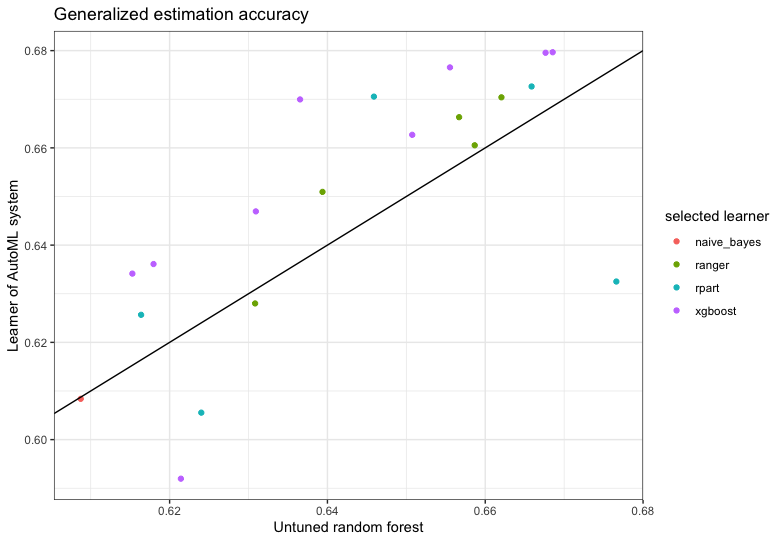
\includegraphics[width=12cm] {image/estimation_accuracy.png}
       \caption{Estimated cross validation accuracy of AutoML learner and untuned random forest seperate per each dataset.}
       \label{acc}
\end{figure}

% latex table generated in R 3.6.2 by xtable 1.8-4 package
% Sun Mar 28 23:40:10 2021
\begin{table}[ht]
\centering
\begin{tabular}{rlrrl}
  \hline
 & Task Dataset & Acc. Automl & Acc. Untuned Random Forest & Sel \\ 
  \hline
  1 & $<$TaskClassif:ATL$>$ & 0.61 & 0.62 & rpart \\ 
  2 & $<$TaskClassif:BOS$>$ & 0.65 & 0.63 & xgboost \\ 
  3 & $<$TaskClassif:DEN$>$ & 0.66 & 0.65 & xgboost \\ 
  4 & $<$TaskClassif:DFW$>$ & 0.63 & 0.68 & rpart \\ 
  5 & $<$TaskClassif:DTW$>$ & 0.63 & 0.62 & rpart \\ 
  6 & $<$TaskClassif:FLL$>$ & 0.61 & 0.61 & naive\_bayes \\ 
  7 & $<$TaskClassif:IAH$>$ & 0.67 & 0.66 & ranger \\ 
  8 & $<$TaskClassif:JFK$>$ & 0.63 & 0.62 & xgboost \\ 
  9 & $<$TaskClassif:LAS$>$ & 0.68 & 0.67 & xgboost \\ 
  10 & $<$TaskClassif:LGA$>$ & 0.65 & 0.64 & ranger \\ 
  11 & $<$TaskClassif:MCO$>$ & 0.63 & 0.63 & ranger \\ 
  12 & $<$TaskClassif:MDW$>$ & 0.68 & 0.67 & xgboost \\ 
  13 & $<$TaskClassif:MEM$>$ & 0.67 & 0.65 & rpart \\ 
  14 & $<$TaskClassif:MIA$>$ & 0.59 & 0.62 & xgboost \\ 
  15 & $<$TaskClassif:PHL$>$ & 0.67 & 0.64 & xgboost \\ 
  16 & $<$TaskClassif:SAN$>$ & 0.68 & 0.66 & xgboost \\ 
  17 & $<$TaskClassif:SEA$>$ & 0.66 & 0.66 & ranger \\ 
  18 & $<$TaskClassif:SFO$>$ & 0.64 & 0.62 & xgboost \\ 
  19 & $<$TaskClassif:SLC$>$ & 0.67 & 0.66 & ranger \\ 
  20 & $<$TaskClassif:STL$>$ & 0.67 & 0.67 & rpart \\ 
   \hline
   \label{acc_table}
   \caption{Estimated cross validation accuracy of AutoML learner and untuned random forest and selected learner per each dataset.}
\end{tabular}
\end{table}

Figure \ref{acc} and table \ref{acc_table} show the accuracy as chosen performance of our AutoML learner for the outer cross-validation and the cross-validated accuracy of the untuned random forest for each dataset. In addition, the selected learner of the AutoML learner applied is color coded over the complete selected dataset in each case in the plot. Points above the line indicate better performance of our learner, points below the line indicate better performance of the untuned random forest.

It can be seen that the AutoML learner ensures a higher accuracy than the untuned random forest for most datasets, but this difference is not huge. In some data sets the AutoML learner performs even worse.

The learner XGBoost was selected most often by our Auto ML system with 9 times out of 20. Consequently, in the future, one might consider committing primarily to this learner for the task of predicting flight delays, and possibly doing more extensive hyperparameter tuning for it.

\subsection{Estimation of performance for new data}
Since the datasets from each airport can be very different, it is difficult to estimate prediction performance on completely new datasets without first having at least a subset of the dataset to train on. As a best estimate in this case, we use the mean of the individually estimated prediction performances over all datasets, which is BLA, with a standard deviation of BLA. Since these estimates do not diverge too much, we also consider this estimate reasonable. 

Other estimates, such as holdout validation of one dataset and training an AutoML learner over all other datasets would also be possible. However, this would require a similarity of the test dataset with the new, unseen datasets and thus is not really a better option.




\section{Conclusion}
It has been shown, using the example of the flight delay prediction task, that an AutoML learner with validation of various machine learning algorithms can tend to lead to improvement in prediction accuracy over an un-tuned standard learner such as Random Forest. However, it should be mentioned that the AutoML learner clearly requires enormously larger resources, both computationally and temporally, and yet the accuracy could not be extremely improved. 

However, this may be due to several reasons. Possibly the selected algorithms, the selected hyperparameters with the selected search spaces as well as the tuner random search were not well or not large enough selected. Possible improvements would be a larger number of learners, hyperparameters and evaluations as well as more complex optimization algorithms with e.g. Bayes Optimization like BOHB or others. However, this again requires far greater resources.

Another possibility is that there is relatively little correlation between the predictors and the target variable in this task. The tendecially rather low accuracies for a binary classification point to such a condition. In this case, even a near-optimal composition of learners, hyperparameters, and optimizers as an AutoML system would not really improve prediction. Accordingly, further benchmarks on other tasks with our AutoML system would be interesting to better estimate the general performance.

However, if the focus is mainly on the given task, there would also be further possibilities to improve the AutoML system, especially with regard to prediction of new, unlabeled data sets. In our benchmark so far, the best learner was determined and stored for each dataset individually. 

One way to use these results would be to combine the choice of trained learners per dataset with unsupervised representation learning or dimension reduction on the individual datasets. Using e.g. kernel PCA or an autoencoder, each dataset, including the new unlabeled ones, could be broken down to a few representative covariates. By e.g. multi-dimensional scaling, distances between the data sets could be calculated.

Using these distances, the most similar labeled record could be determined for the unlabeled records and its learner adopted. If there are only few labeled data or if they are added in the course of time, the learner could serve as a starting point for further hyperparameter tuning.

A benchmark of this idea, preferably in combination with the further improvement of the AutoML learner itself could be an interesting and, above all, application-oriented research opportunity.

\nocite{*}
\bibliography{literature.bib}
\end{document}
